\documentclass[10pt,a4paper]{article}
%\usepackage[ngerman]{babel}
\usepackage{color}
\usepackage{listings}
\usepackage{graphicx}
\usepackage{float}
%\usepackage{moreverb}
\usepackage[section]{placeins}

\setlength{\parindent}{0pt}

\title{\textbf{Shape Matching with Earth Mover's Distance}}
\author{Jon Volkmar\\
		Mart\'{i} Griera}
\date{}
\begin{document}

\maketitle

\section{Introduction}

\section{Experiment Setup}

\begin{figure}[ht!]
\centering
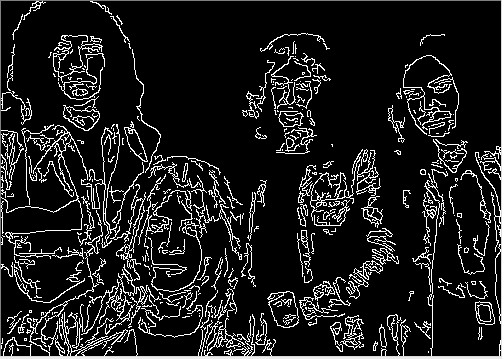
\includegraphics{canny_edge.png}
\caption{Output of Canny edge detector - edges are marked with a white outline}
\label{overflow}
\end{figure}

\begin{figure}[ht!]
\centering
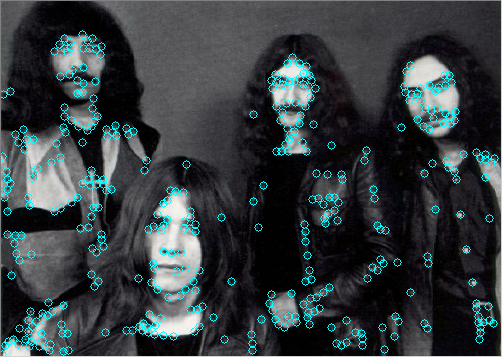
\includegraphics{harris_corner.png}
\caption{Harris Corner Detection - Detected corners are marked with blue circles}
\label{overflow}
\end{figure}

\begin{figure}[ht!]
\centering
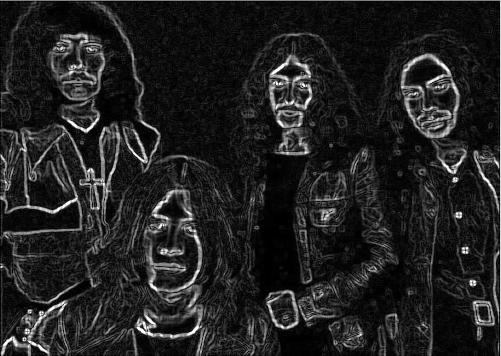
\includegraphics{sobel_intensity_gradient.png}
\caption{Image of the magnitude of the intensity gradient, calculated using the Sobel operator}
\label{overflow}
\end{figure}

\begin{figure}[ht!]
\centering
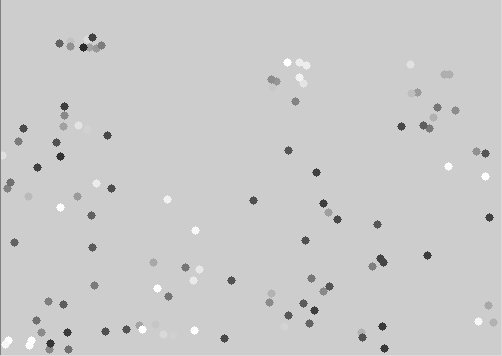
\includegraphics{weighted_point_set.png}
\caption{Each corner that is on a detected edge is given a weight, corresponding to the intensity gradient value at the same location, giving us a weighted point set. Low weights are black, high weights are white.}
\label{overflow}
\end{figure}

\section{Preliminary Results}



\end{document}